\def\made{0102}
\begin{name}
	{Biên soạn \& Phản biện: Nhóm 2}
	{Đề thi chính thức}
\end{name}
\Opensolutionfile{ansbook}[ans/ansb\currfilebase]
\caulc
\Opensolutionfile{ans}[ans/ans\currfilebase-Phan-I]
\begin{ex}%[Dự án 50QMBB-VN-MT-15+]%[2-TN-0102-BGD-2026,VM038]%[2H2N1-1]
	\immini[thm]{Cho hình lập phương $ABCD.A'B'C'D'$ (xem hình vẽ). Vectơ nào sau đây bằng vectơ $\overrightarrow{AD}$?
		\choice[2]
			{$\overrightarrow{AB}$}
			{$\overrightarrow{AA'}$}
			{$\overrightarrow{CD}$}
			{\True $\overrightarrow{B'C'}$}
		}{
		\begin{tikzpicture}[scale=0.8, font=\footnotesize, line join=round, line cap=round, >=stealth]
    %hidden: VM005
			\def\a{3}
			\def\b{2}
			\def\h{3}
			\path 	(0:0) coordinate (A)
				++(0:\a) coordinate (B)
				++(-135:\b) coordinate (C)
				($(A)+(C)-(B)$) coordinate (D)
				($(A)+(90:\h)$) coordinate (A')
				($(B)+(90:\h)$) coordinate (B')
				($(C)+(90:\h)$) coordinate (C')
				($(D)+(90:\h)$) coordinate (D');
			\draw[dashed] 	(D)--(A)--(B)	(A)--(A');
			\draw	(C)--(C') 	(D)--(D') 	(B)--(B')	(C)--(C')
				(B)--(C)--(D) 
				(A')--(B')--(C')--(D')--cycle;
			\foreach \x/\g in {A/150,D/225,C/-45,B/0,A'/135,D'/180,C'/-30,B'/45}
			\fill (\x) circle (1pt)
				($(\g:3.5mm)+(\x)$) node {$\x$};	
    \node at (0,0){\href{50QMBB}{\tiny \phantom{50QMBB}}};
		\end{tikzpicture}
		}	
	\loigiai{
		Vì  $ABCD.A'B'C'D'$ là hình lập phương nên $\overrightarrow{AD}=\overrightarrow{B'C'}$.
	}
\end{ex}

\begin{ex}%[Dự án 3YND5G-VN-MT-15+]%[2-TN-0102-BGD-2026,VM038]%[1D7N2-1] 
	Cho các hàm số $y=f(x)$ và $y=g(x)$ có đạo hàm trên tập số thực $\mathbb{R}$ thỏa mãn
	$f'(x)=2x$, $g'(x)=x^2$. Đạo hàm của hàm số $y=f(x)+g(x)$ là
	\choice
		{$4x$}
		{\True $2x+x^2$}
		{$2+2x$}
		{$2+x^2$}
	\loigiai{
		Ta có $\big(f(x)+g(x)\big)'= f'(x)+g'(x)= 2x+x^2$.
	}
\end{ex}

\begin{ex}%[Dự án JLR58L-VN-MT-15+]%[2-TN-0102-BGD-2026,VM038]%[2H2N2-3]
	Trong không gian với hệ tọa độ $Oxyz$, cho hai điểm	$A(2;3;1)$ và $B(4;1;1)$.
	Vectơ $\overrightarrow{AB}$ có tọa độ là
	\choice
		{$(3;2;1)$}
		{$(-2;2;0)$}
		{$(6;4;2)$}
		{\True $(2;-2;0)$}	
	\loigiai{
		Ta có $\overrightarrow{AB}=(2;-2;0)$.
	}
\end{ex}

\begin{ex}%[Dự án 4CMN6C-VN-MT-15+]%[2-TN-0102-BGD-2026,VM038]%[2D4H1-1] 
	Cho $\displaystyle	\int f(x)\mathrm{\,d} x=\sin x+C$. Phát biểu nào sau đây đúng?
	\choice
		{$\displaystyle\int\big[2+f(x)\big]\mathrm{d} x=2x-\sin x+C$}
		{\True $\displaystyle\int\big[2+f(x)\big]\mathrm{d} x=2x+\sin x+C$}
		{$\displaystyle\int\big[2+f(x)\big]\mathrm{d} x=2x+\cos x+C$}
		{$\displaystyle\int\big[2+f(x)\big]\mathrm{d} x=2x-\cos x+C$}
	\loigiai{
		Theo tính chất của nguyên hàm,
		\[
		\displaystyle\int\big[2+f(x)\big]\mathrm{d} x
		=\displaystyle\int2\mathrm{\,d} x+\displaystyle\int f(x)\mathrm{\,d} x=2x+\sin x+C.
		\]
	}
\end{ex}

\begin{ex}%[Dự án 2VOV09-VN-MT-15+]%[2-TN-0102-BGD-2026,VM038]%[1D2N3-4]
	Cho cấp số nhân $(u_n)$ có số hạng đầu $u_1$ và công bội $q$ với $u_1\ne 0$, $q>1$. Số hạng $u_3$ là
	\choice
		{$u_3=u_1\cdot q^3$}
		{$u_3=u_1+2q$}
		{\True $u_3=u_1\cdot q^2$}
		{$u_3=u_1+3q$}
	\loigiai{
		Ta có $u_3=u_1\cdot q^{3-1}=u_1\cdot q^2$.		
	}
\end{ex}

\begin{ex}%[Dự án 2FZ8F0-VN-MT-15+]%[2-TN-0102-BGD-2026,VM038]%[1D6H4-2]
	Nghiệm của phương trình	$\log_3(3x)=2$ là
	\choice
		{$x=2$}
		{\True $x=3$}
		{$x=\dfrac{8}{3}$}
		{$x=\dfrac{2}{3}$}
	\loigiai{
		Ta có $\log_3(3x)=2 \Leftrightarrow 3x=3^2\Leftrightarrow x=3$.
	}
\end{ex}

\begin{ex}%[Dự án 3PC0ZD-VN-MT-15+]%[2-TN-0102-BGD-2026,VM038]%[1D2N2-4]
	Cho cấp số cộng $(u_n)$ có $u_1=-2$ và công sai $d=3$. Giá trị của $u_2$ bằng
	\choice
		{\True $1$}
		{$-1$}
		{$-6$}
		{$-5$}
	\loigiai{
		Ta có $u_2=u_1+d=-2+3=1$.
	}
\end{ex}

\begin{ex}%[Dự án 66MO7B-VN-MT-15+]%[2-TN-0102-BGD-2026,VM038]%[2D4N1-1] 
	Hàm số $F(x)=5x^3$ là một nguyên hàm của hàm số nào sau đây?
	\choice
		{$f_2(x)=5x^2$}
		{$f_4(x)=5x^4$}
		{\True $f_3(x)=15x^2$}
		{$f_1(x)=\dfrac{5x^4}{4}$}
	\loigiai{
		Ta có $F'(x)=\left( 5x^3\right)'=15x^2$.\\
		Vậy $F(x)$ là một nguyên hàm của $f_3(x)=15x^2$.
	}
\end{ex}

\begin{ex}%[Dự án 2PR8M5-VN-MT-15+]%[2-TN-0102-BGD-2026,VM038]%[1D9N1-3] 
	Cho hai biến cố độc lập $A$ và $B$ có xác suất $\mathrm{P}(A)=0{,}3$ và $\mathrm{P}(B)=0{,}6$.	Giá trị của $\mathrm{P}(AB)$ bằng
	\choice
		{$0{,}9$}
		{$0{,}3$}
		{\True $0{,}18$}
		{$0{,}5$}
	\loigiai{
		Vì $A$ và $B$ độc lập nên
		\[	\mathrm{P}(AB)=\mathrm{P}(A)\cdot\mathrm{P}(B)=0{,}3\cdot 0{,}6=0{,}18.\]
	}
\end{ex}

\begin{ex}%[Dự án 5ZR5JC-VN-MT-15+]%[2-TN-0102-BGD-2026,VM038]%[0D2N2-1]
	Cặp số nào sau đây là một nghiệm của hệ bất phương trình $\heva{
	&x+y-2<0\\
	&x-y+2>0}$?
	\choice
		{\True $(1;0)$}
		{$(0;3)$}
		{$(-3;0)$}
		{$(1;2)$}	
	\loigiai{
		Xét các cặp số $(1;0)$, $(0;3)$, $(-3;0)$, $(1;2)$:
		\begin{itemize}
			\item Vì $1+0-2=-1<0$ và $1-0+2=3>0$ nên cặp số $(1;0)$ là một nghiệm của hệ bất phương trình đã cho.
			\item Vì $0+3-2=1>0$ và $0-3+2=-1<0$ nên cặp số $(0;3)$ không phải là nghiệm của hệ bất phương trình đã cho.
			\item Vì $-3+0-2=-5<0$ và $-3-0+2=-1<0$ nên cặp số $(-3;0)$ không phải là nghiệm của hệ bất phương trình đã cho.
			\item Vì $1+2-2=1>0$ và $1-2+2=1>0$ nên cặp số $(1;2)$ không phải là nghiệm của hệ bất phương trình đã cho.
		\end{itemize}
		Vậy  cặp số $(1;0)$ là một nghiệm của hệ bất phương trình đã cho.
	}
\end{ex}

\begin{ex}%[Dự án 51F0BA-VN-MT-15+]%[2-TN-0102-BGD-2026,VM038]%[1D5N2-2]
	Khảo sát thời gian (đơn vị: phút) học trực tuyến trong một ngày của $42$ học sinh, người ta thu được mẫu số liệu ghép nhóm sau:
	\begin{center}
		\begin{tabular}{|c|c|c|c|c|c|c|}
			\hline
			Thời gian học trực tuyến&$[10;20)$ & $[20;30)$ &$[30;40)$ &$[40;50)$ &$[50;60)$ &$[60;70)$\\
			\hline
			Số học sinh &$5$ &$7$ &$15$ &$6$ &$5$ &$4$\\
			\hline
		\end{tabular}
	\end{center}
	Trung vị của mẫu số liệu thuộc nhóm nào sau đây?
	\choice
		{$[40;50)$}
		{$[20;30)$}
		{\True $[30;40)$}
		{$[50;60)$}
	\loigiai{
		Ta có	$\dfrac{42}{2}=21$.\\
		Số hạng thứ $21$ và $22$ đều nằm trong nhóm $[30;40)$.\\
		Vậy trung vị thuộc nhóm $[30;40)$.
	}
\end{ex}

\begin{ex}%[Dự án 5CSMV2-VN-MT-15+]%[2-TN-0102-BGD-2026,VM038]%[2D1N4-1]
	Cho hàm số	$y=\dfrac{ax+b}{cx+d}$ ($c\ne0$, $\ ad-bc\ne0$) có bảng biến thiên như hình dưới đây:
	\begin{center}
		\begin{tikzpicture}
    %hidden: VM005
			\tkzTabInit[nocadre=true, lgt=1, espcl=4, deltacl=0.5]
			{$x$/0.7,$y'$/0.7,$y$/2}
			{$-\infty$,$1$,$+\infty$}
			\tkzTabLine{,+,d,+,}
			\tkzTabVar{-/$-2$,+D-/$+\infty$/$-\infty$,+/$-2$}
    \node at (T11){\href{5CSMV2}{\tiny \phantom{5CSMV2}}};
		\end{tikzpicture}
	\end{center}
	Đường tiệm cận đứng của đồ thị hàm số đã cho có phương trình là
	\choice
		{$x=-2$}
		{$y=1$}
		{$y=-2$}
		{\True $x=1$}
	\loigiai{
		Quan sát bảng biến thiên, ta thấy 
		\[\lim\limits_{x\to 1^-} y=+\infty, \lim\limits_{x\to 1^+} y=-\infty \]
		Do đó phương trình tiệm cận đứng là $x=1$.
	}
\end{ex}

\Closesolutionfile{ans}
\cauds
\Opensolutionfile{ans}[ans/ans\currfilebase-Phan-II]
\begin{ex}%[Dự án 4DPQGO-VN-MT-15+]%[2-TN-0102-BGD-2026,VM012]%[2D4V2-6]
	Một hệ thống pin năng lượng mặt trời gồm các tấm pin được kết nối với một bộ lưu trữ điện. Trong thời gian mặt trời chiếu sáng của một ngày, năng lượng điện thu được từ các tấm pin được lưu trong bộ lưu trữ điện. Gọi $F(t)$ là năng lượng điện (kWh) lưu trữ được kể từ thời điểm hệ thống bắt đầu hoạt động đến thời điểm $t$, trong đó $t$ là thời gian tính theo giờ ($0 \le t \le 12$) và thời điểm hệ thống bắt đầu hoạt động ứng với $t=0$. Biết rằng $F(0)=0$.\\
	\noindent Tốc độ lưu trữ năng lượng điện (kW) của hệ thống này là hàm số $f(t)=F'(t)$ với $0 \le t \le 12$. Số liệu ghi nhận được ở một ngày cụ thể trong năm cho thấy $f(t)=-0{,}15t^2+1{,}8t$ với $0 \le t \le 12$.
	\choiceTF
		{\True $F(t)=-0{,}05t^3+0{,}9t^2$ với $0 \le t \le 12$}
		{\True Năng lượng điện (kWh) lưu trữ được kể từ thời điểm $t=a$ đến thời điểm $t=b$ ($0 \le a < b \le 12$) là $\displaystyle\int\limits_a^b f(t)\mathrm{\,d}t$}
		{Năng lượng điện lưu trữ được kể từ thời điểm $t=1$ đến thời điểm $t=5$ nhỏ hơn $15{,}3$ kWh}
		{Năng lượng điện lưu trữ được kể từ thời điểm $t=1$ đến thời điểm $t=9$ gấp hai lần năng lượng điện lưu trữ được kể từ thời điểm $t=1$ đến thời điểm $t=5$}
	\loigiai{
		\begin{itemchoice}
			\itemch Ta có $\displaystyle\int f(t) \mathrm{\,d}t = \displaystyle\int \left( -0{,}15t^2 + 1{,}8t\right)\mathrm{d}t = -0{,}05t^3 + 0{,}9t^2 + C$. \\
			Vì $F(t)$ là một nguyên hàm của $f(t)$ trên đoạn $[0;12]$ nên $F(t) = -0{,}05t^3 + 0{,}9t^2 + C \text{ với } 0 \le t \le 12$.\\
			Mà $F(0) = 0 \Rightarrow C = 0$. Do đó $F(t) = -0{,}05t^3 + 0{,}9t^2$ với $0 \le t \le 12$.
			\itemch Vì $f(t)=F'(t)$ là tốc độ lưu trữ năng lượng điện nên năng lượng điện lưu trữ được kể từ thời điểm $t=a$ đến thời điểm $t=b$ ($0 \le a<b \le 12$) là 
			\[F(b) - F(a) = \displaystyle\int\limits_a^b F'(t)\mathrm{\,d}t = \displaystyle\int\limits_a^b f(t)\mathrm{\,d}t.\]
			\itemch Năng lượng điện lưu trữ được kể từ thời điểm $t=1$ đến thời điểm $t=5$ là
			\begin{align*}
				\Delta F_1 &= F(5) - F(1) \\
				&= \left(-0{,}05 \cdot 5^3 + 0{,}9 \cdot 5^2\right) - \left(-0{,}05 \cdot 1^3 + 0{,}9 \cdot 1^2\right) \\
				&= 16{,}25 - 0{,}85 = 15{,}4 \text{ (kWh)}.
			\end{align*}
			Vì $15{,}4 > 15{,}3$ nên mệnh đề này sai.
			\itemch Năng lượng điện lưu trữ được kể từ thời điểm $t=1$ đến thời điểm $t=9$ là
			\begin{align*}
				\Delta F_2 &= F(9) - F(1) \\
				&= \left(-0{,}05 \cdot 9^3 + 0{,}9 \cdot 9^2\right) - 0{,}85 \\
				&= 36{,}45 - 0{,}85 = 35{,}6 \text{ (kWh)}.
			\end{align*}
			Ta thấy $35{,}6 \neq 2 \cdot 15{,}4$, do đó mệnh đề này sai.
		\end{itemchoice}
	}
\end{ex}

\begin{ex}%[Dự án 5BS27X-VN-MT-15+]%[2-TN-0102-BGD-2026,VM012]%[2D1H2-1]
	Cho hàm số $f(x)=\dfrac{1}{3}x^3-2x^2+3x+8$.
	\choiceTF
		{\True Đạo hàm của hàm số đã cho là $f'(x)=x^2-4x+3$}
		{\True Phương trình $f'(x)=0$ có tập nghiệm là $S=\{1;3\}$}
		{\True Hàm số đã cho nghịch biến trên khoảng $(1;3)$}
		{Giá trị cực tiểu của hàm số đã cho bằng $\dfrac{28}{3}$}
	\loigiai{
		\begin{itemchoice}
			\itemch Ta có $f'(x) = \left(\dfrac{1}{3}x^3 - 2x^2 + 3x + 8\right)' = x^2 - 4x + 3$.
			\itemch Xét phương trình $f'(x) = 0 \Leftrightarrow x^2 - 4x + 3 = 0 \Leftrightarrow \hoac{&x = 1\\&x = 3.}$ \\
			Vậy tập nghiệm của phương trình là $S = \{1; 3\}$.
			\itemch Bảng biến thiên
			\begin{center}
				\begin{tikzpicture}
    %hidden: VM005
					\tkzTabInit[nocadre=true,lgt=1.2,espcl=3.0,deltacl=0.5]
					{$x$/0.7, $f'(x)$/0.7, $f(x)$/2}
					{$-\infty$,$1$,$3$,$+\infty$}
					\tkzTabLine{,+,0,-,0,+,}
					\tkzTabVar{-/$-\infty$, +/$\dfrac{28}{3}$, -/$8$, +/$+\infty$}
    \node at (T11){\href{5BS27X}{\tiny \phantom{5BS27X}}};
				\end{tikzpicture}
			\end{center}
			Dựa vào bảng biến thiên, hàm số nghịch biến trên khoảng $(1; 3)$.
			\itemch Hàm số đạt cực tiểu tại $x = 3$, giá trị cực tiểu của hàm số đã cho bằng $8$.
		\end{itemchoice}
	}
\end{ex}

\begin{ex}%[Dự án 5LYC03-VN-MT-15+]%[2-TN-0102-BGD-2026,TV028]%[2D6H1-2]
	Nhằm đưa ra cảnh báo sớm về tình trạng sức khỏe của cư dân, người ta sử dụng một ứng dụng trí tuệ nhân tạo để sàng lọc nguy cơ mắc bệnh dựa trên hồ sơ y tế được lưu trữ. Khi phát hiện nguy cơ mắc bệnh, ứng dụng này sẽ gửi cảnh báo để giúp người dân đi khám bệnh kịp thời. Người ta dùng ứng dụng này để tầm soát nguy cơ mắc một loại bệnh.\\
	Kết quả thu được khi quét thử nghiệm hồ sơ y tế của $10\,000$ người như sau: Có $1\,000$ người nhận được cảnh báo và $9\,000$ người còn lại không nhận được cảnh báo từ ứng dụng. Trong số $1\,000$ người nhận được cảnh báo thì có $600$ người có bệnh và $400$ người không có bệnh. Trong số $9\,000$ người không nhận được cảnh báo thì có $200$ người có bệnh và $8\,800$ người không có bệnh.\\
	Chọn ngẫu nhiên một người trong số $10\,000$ người nói trên.
	\choiceTF
		{\True Xác suất để người đó không nhận được cảnh báo từ ứng dụng bằng $0{,}9$}
		{\True Xác suất để người đó không có bệnh, biết rằng người đó không nhận được cảnh báo từ ứng dụng, lớn hơn $0{,}97$}
		{Xác suất để người đó không có bệnh bằng $0{,}9$}
		{\True Xác suất để người đó không nhận được cảnh báo từ ứng dụng, biết rằng người đó không có bệnh, lớn hơn $0{,}95$}
	\loigiai{
		Gọi $A$ là biến cố \lq\lq người đó nhận được cảnh báo từ ứng dụng\rq\rq.\\
		Suy ra biến cố đối $\overline{A}$ là \lq\lq người đó không nhận được cảnh báo từ ứng dụng\rq\rq.\\
		Gọi $B$ là biến cố \lq\lq người đó có bệnh\rq\rq, suy ra $\overline{B}$ là biến cố \lq\lq người đó không có bệnh\rq\rq.\\
		Số phần tử của không gian mẫu là $n(\Omega) = 10\,000$. Theo giả thiết, ta có
		\begin{itemize}
			\item $n(A) = 1\,000$ và $n\left(\overline{A}\right) = 9\,000$.
			\item $n(AB) = 600$ và $n\left(A\overline{B}\right) = 400$.
			\item $n\left(\overline{A}B\right) = 200$ và $n\left(\overline{A}\, \overline{B}\right) = 8\,800$.
		\end{itemize}
		Biểu đồ Ven sau đây mô tả quan hệ giữa các biến cố trên:
		\begin{center}
			\begin{tikzpicture}[scale=1, font=\footnotesize, line join=round, line cap=round, >=stealth]				
    %hidden: VM005
				\def\firstven{(0,0) ellipse (1.5cm and 1cm)}				
				\def\secondven{(1.8,0) ellipse (1.5cm and 1cm)}
				\def\hcn{(-2,-2.2) rectangle (4,1.4) node[below left]{$\Omega$} }
				\begin{scope}
					\clip \firstven;
					\clip \secondven;
					\fill[pattern=north east lines,opacity=0.4] \secondven;
				\end{scope}
				\draw \firstven \secondven;%\thirdven;
				\draw \hcn;
				\draw (3.2,-0.8)node{$B$} (-1.5,-0.8)node{$A$} (0.85,0.25)node{$AB$}
					(0.85,-0.25)node{$600$} 
					(2.3,0.25)node{$\overline{A}B$}
					(2.3,-0.25)node{$200$}
					(-0.3,0.25)node{$A\overline{B}$} (-0.3,-0.25)node{$400$}
					(0.5,-1.4)node{$\overline{A}\, \overline{B}$}
					(0.5,-1.9)node{$8\,800$};
    \node at (0,0){\href{5LYC03}{\tiny \phantom{5LYC03}}};
			\end{tikzpicture}
		\end{center}
		\begin{itemchoice}
			\itemch Xác suất để người đó không nhận được cảnh báo là $\mathrm{P}\left(\overline{A}\right) = \dfrac{n\left(\overline{A}\right)}{n(\Omega)} = \dfrac{9\,000}{10\,000} = 0{,}9$.
			\itemch Xác suất để người đó không có bệnh, biết rằng người đó không nhận được cảnh báo là \[\mathrm{P}\left(\overline{B} \mid \overline{A}\right) = \dfrac{n\left(\overline{A}\, \overline{B}\right)}{n\left(\overline{A}\right)} = \dfrac{8\,800}{9\,000} = \dfrac{44}{45} \approx 0{,}978 > 0{,}97.\]
			\itemch Tổng số người không có bệnh là \[n\left(\overline{B}\right) = n\left(A \overline{B}\right) + n\left(\overline{A}\, \overline{B}\right) = 400 + 8\,800 = 9\,200.\]
			Xác suất để người đó không có bệnh là $\mathrm{P}\left(\overline{B}\right) = \dfrac{n\left(\overline{B}\right)}{n(\Omega)} = \dfrac{9\,200}{10\,000} = 0{,}92 \neq 0{,}9$.
			\itemch Xác suất để người đó không nhận được cảnh báo, biết rằng người đó không có bệnh là \[\mathrm{P}\left(\overline{A} \mid \overline{B}\right) = \dfrac{n\left(\overline{A}\, \overline{B}\right)}{n\left(\overline{B}\right)} = \dfrac{8\,800}{9\,200} = \dfrac{22}{23} \approx 0{,}9565 > 0{,}95.\]
		\end{itemchoice}
	}
\end{ex}

\begin{ex}%[Dự án 2D5424-VN-MT-15+]%[2-TN-0102-BGD-2026,TV028]%[2H5V2-8]
	Trong không gian xét hệ tọa độ $Oxyz$ có một đơn vị dài trên các trục tương ứng với $10$ mét trên thực tế. Một mục tiêu cần được bảo vệ có vị trí ở gốc tọa độ $O$. Người ta thiết lập một vành đai bảo vệ quanh mục tiêu theo một đường tròn tâm $O$ có bán kính bằng $6$ đơn vị (tương ứng $60$ mét trên thực tế) nằm trong mặt phẳng $(Oxy)$. Một máy bay không người lái (được coi như một hạt) bay theo một đường thẳng từ vị trí $M(2; 11; 3)$ đến vị trí $N(14; 2; 3)$. Tại mỗi vị trí của máy bay, khoảng cách từ máy bay đến vành đai bảo vệ là độ dài ngắn nhất của các đoạn thẳng nối từ vị trí đó đến một điểm bất kì trên vành đai.
	\choiceTF
		{\True $\overrightarrow{MN}=(12;-9; 0)$}
		{Phương trình tham số của đường thẳng $MN$ là $\heva{&x=2+4t \\ &y=11-3t \\ &z=0}$ với $t \in \mathbb{R}$}
		{Trong quá trình bay từ $M$ đến $N$, khoảng cách ngắn nhất từ máy bay đến vành đai bảo vệ là $100$ mét}
		{\True Trong quá trình bay từ $M$ đến $N$, khoảng cách từ máy bay đến vành đai bảo vệ là ngắn nhất khi máy bay ở vị trí có tọa độ là $(6; 8; 3)$}
	\loigiai{
		\begin{itemchoice}
			\itemch Ta có vectơ $\overrightarrow{MN} = (14 - 2; 2 - 11; 3 - 3) = (12; -9; 0)$.
			\itemch Đường thẳng $MN$ đi qua điểm $M(2; 11; 3)$, có vectơ chỉ phương $\overrightarrow{u}= (4; -3; 0)$ (do $\overrightarrow{u}=\dfrac{1}{4}\overrightarrow{MN}$) nên có phương trình tham số là $\heva{&x = 2 + 4t \\ &y = 11 - 3t \\ &z = 3}$ với $t \in \mathbb{R}$.
			\itemch Gọi $H$ là vị trí của máy bay trên đoạn thẳng $MN$ thì $H(x; y; 3)$. \\
			Gọi $M'$, $N'$, $K$ lần lượt là hình chiếu vuông góc của $M$, $N$, $H$ lên mặt phẳng $(Oxy)$. Khi đó $M'(2; 11; 0)$, $N'(14; 2; 0)$, $K(x; y; 0)$ và $HK=3$.\\
			Gọi vành đai bảo vệ, tức đường tròn tâm $O$, bán kính $R=6$ nằm trong mặt phẳng $(Oxy)$ là $\mathscr{(C)}$. Xét điểm $P$ bất kỳ thuộc $\mathscr{(C)}$ (xem hình $1$).
			\begin{center}
				\begin{tikzpicture}[scale=0.9, font=\footnotesize, line join=round, line cap=round, >=stealth, x={(-0.3cm, -0.2cm)}, y={(0.4cm, 0cm)}, z={(0cm, 0.5cm)}]
    %hidden: VM005
					\draw[->] (0,0,0) -- (15,0,0) node[above] {$x$};
					\draw[->] (0,0,0) -- (0,12,0) node[below] {$y$};
					\draw[->] (0,0,0) -- (0,0,4.5) node[left] {$z$};
					\coordinate (O) at (0,0,0);
					\coordinate (M) at (2,11,3);
					\coordinate (N) at (14,2,3);
					\coordinate (Mp) at (2,11,0);
					\coordinate (Np) at (14,2,0);
					\coordinate (H) at (6,8,3);
					\coordinate (K) at (6,8,0);
					\coordinate (P) at (3.6,4.8,0);
					\draw plot[domain=0:360, samples=100] ({6*cos(\x)}, {6*sin(\x)}, 0);
					\draw[dashed] (M) -- (Mp)  (N) -- (Np) (H) -- (K) (O) -- (K);
					\draw (Mp) -- (Np);
					\draw[red] (M) -- (N);
					\draw[teal] (H) -- (P);
					\fill (O) circle (1pt) node[above left] {$O$}
						(M) circle (1pt) node[above right] {$M$}
						(N) circle (1pt) node[above left] {$N$}
						(Mp) circle (1pt) node[below right] {$M'$}
						(Np) circle (1pt) node[below] {$N'$}
						(H) circle (1pt) node[above] {$H$}
						(K) circle (1pt) node[below right] {$K$}
						(P) circle (1pt) node[below] {$P$};
					\pic [draw, angle radius=2mm] {right angle = P--K--H};
					\node at ({6*cos(175)}, {6*sin(175)}, 0) [above] {$\mathscr{(C)}$};
					\node at ($(O)+(0,0,-7)$) {Hình $1$};
    \node at (0,0){\href{2D5424}{\tiny \phantom{2D5424}}};
				\end{tikzpicture}
				\qquad
				\begin{tikzpicture}[scale=0.9, font=\footnotesize, line join=round, line cap=round, >=stealth,x=0.5cm,y=0.5cm]
    %hidden: VM005
				  \pgfmathsetmacro{\Radius}{3} 
				  \pgfmathsetmacro{\PosK}{0.65}
				  \pgfmathsetmacro{\Ext}{0.15}
				  \def\xmin{-3.5} \def\xmax{8} \def\ymin{-3.5} \def\ymax{6.5}      
				  \coordinate (O) at (0,0);
				  \coordinate (M) at (1,5.5);
				  \coordinate (N) at (7,1);
				  \coordinate (K0) at ($(M)!(O)!(N)$);
				  \coordinate (K) at ($(M)!{\PosK}!(N)$);
				  \draw[->] (\xmin, 0) -- (\xmax+1, 0) node[below] {$x$};
				  \draw[->] (0, \ymin) -- (0, \ymax+0.5) node[left] {$y$};
				  \draw[name path=circle] (O) circle (\Radius);
				  \draw[dashed] ($(M)!-\Ext!(N)$) -- ($(M)!1+\Ext!(N)$); 
				  \draw (M) -- (N);      
				  \path[name path=lineOK] (O) -- (K);
				  \path[name path=lineOK0] (O) -- (K0);
				  \path[name intersections={of=circle and lineOK, by=P}];
				  \path[name intersections={of=circle and lineOK0, by=P0}];
				  \draw (O) -- (K0) (O) -- (K);
				  \draw[dashed] (1,0)|-(0,5.5) (7,0)|-(0,1);
				  \pic [draw, angle radius=2mm] {right angle = O--K0--M};
				  \foreach \p/\ang/\label in {O/225/O, M/45/M', N/45/N', K0/45/K_0, K/45/K, P/60/P, P0/100/P_0%
				  }{
				   \fill[black] (\p) circle (1pt);
				   \node[shift={(\ang:0.3cm)}] at (\p) {$\label$};
				  }
				  \foreach \x/\y/\ang/\label in {1/0/-90/2, 0/5.5/180/11, 7/0/-90/14, 0/1/180/2,3/0/-60/6
				  }{
				   \fill (\x,\y) circle (1pt);
				   \node[shift={(\ang:0.3cm)}] at (\x,\y) {$\label$};
				  }      
					\node at ($(O)+(0,-4.5)$) {Hình $2$};
    \node at (0,0){\href{2D5424}{\tiny \phantom{2D5424}}};
				 \end{tikzpicture}
			\end{center}
			Vì tam giác $PHK$ vuông tại $K$ nên khoảng cách $HP$ là \[HP = \sqrt{HK^2 + KP^2} = \sqrt{3^2 + KP^2}=\sqrt{9 + (OK-R)^2}=\sqrt{9 + (OK-6)^2}.\]
			Để $HP$ nhỏ nhất thì độ dài đoạn thẳng $OK$ phải nhỏ nhất, tức là $K$ ở vị trí $K_0$ là hình chiếu vuông góc của $O$ lên đoạn thẳng $M'N'$.\\
			Xét trong mặt phẳng $(Oxy)$: (xem hình $2$)\\
			Đường thẳng $M'N'$ đi qua $M'(2; 11)$ và $N'(14; 2)$ có phương trình là
			\[\dfrac{x - 2}{14-2}= \dfrac{y - 11}{2-11} = 0 \Leftrightarrow 3x + 4y - 50 = 0.\]
			Khoảng cách từ $O(0; 0)$ đến đường thẳng $M'N'$ là \[OK_0= \dfrac{|3 \cdot 0 + 4 \cdot 0 - 50|}{\sqrt{3^2 + 4^2}} = 10.\]
			Khoảng cách ngắn nhất của đoạn thẳng $HP$ là 
			\[d = \sqrt{9 + (OK_0-6)^2}= \sqrt{3^2 + (10 - 6)^2} = 5\ (\text{đơn vị}).
			\]
			Vậy khoảng cách ngắn nhất từ máy bay đến vành đai bảo vệ là $50$ mét.		
			\itemch Máy bay đạt khoảng cách ngắn nhất khi $K$ di chuyển đến vị trí của $K_0$, với $K_0$ là hình chiếu vuông góc của $O$ lên đường thẳng $M'N'$.\\
			Trong mặt phẳng $(Oxy)$, đường thẳng $OK_0$ đi qua $O$ và vuông góc với $M'N'$ có phương trình là $4x - 3y = 0$.\\
			Tọa độ điểm $K_0$ là nghiệm của hệ phương trình $\heva{&3x + 4y - 50 = 0 \\ &4x - 3y = 0} \Leftrightarrow \heva{&x = 6 \\ &y = 8}$.\\
			Từ đó suy ra trong không gian $Oxyz$, điểm $K_0$ có tọa độ là $(6; 8; 0)$. Do đó $H(6; 8; 3)$.\\
			Ta thấy hoành độ $x_H = 6$ thỏa mãn $2 \le x_H \le 14$ nên điểm $H$ nằm trên đoạn thẳng $MN$.\\
			Vậy khoảng cách từ máy bay đến vành đai bảo vệ là ngắn nhất khi máy bay ở vị trí có tọa độ là $(6; 8; 3)$.
		\end{itemchoice}
	}
\end{ex}

\Closesolutionfile{ans}
\caukq
\Opensolutionfile{ans}[ans/ans\currfilebase-Phan-III]
\begin{ex}%[Dự án 2BBI0A-VN-MT-15+]%[2-TN-0102-BGD-2026,VM026]%[2D4V3-5]
	Để chế tác một hạt cườm, người ta lấy một khối vật thể có dạng một khối tròn xoay được tạo thành khi quay hình phẳng giới hạn bởi trục $Ox$ và nửa trên của elip $\dfrac{x^2}{1{,}5^2} + \dfrac{y^2}{1^2} = 1$ (một đơn vị dài trên mỗi trục tọa độ tương ứng với một xăng-ti-mét trong thực tế) quanh trục $Ox$; sau đó khoan dọc theo trục xoay (xem hình dưới). Lỗ khoan có dạng hình trụ với bán kính $0{,}1$\,cm và có trục nằm trên trục xoay. Phần còn lại sau khi khoan là hạt cườm, có dạng một khối tròn xoay.\\
	Thể tích của hạt cườm đó bằng bao nhiêu xăng-ti-mét khối (\textit{không làm tròn kết quả các phép tính trung gian, chỉ làm tròn kết quả cuối cùng đến hàng phần trăm})?
	\begin{center}
		\begin{tikzpicture}[font=\footnotesize, >=stealth, line join=round, line cap=round, scale=1.0]			
    %hidden: VM005
			\def\h{0.3} 
			\def\xx{1.42} 				
			% --- Hình 1 
			\begin{scope}
				\draw(-2.2,0) -- (-1.5,0);
				\draw[dashed] (-1.5,0) -- (1.5,0);
				\draw[->] (1.5,0) -- (2.2,0) node[below] {$x$};
				\draw (0,-1.4) -- (0,-1);
				\draw[dashed] (0,-1) -- (0,1);
				\draw[->] (0,1) -- (0,1.6) node[below left] {$y$};
				\fill (0,0) node{\href{2BBI0A}{\tiny \phantom{2BBI0A}}} node[shift={(-150:1.8ex)}]{$O$} circle(1pt);	
				\draw (0,0) ellipse (1.5 and 1);
				\draw[dashed] (-\xx,\h) -- (\xx,\h);
				\draw[dashed] (-\xx,-\h) -- (\xx,-\h);					
				\draw (0,-1) arc (-90:90:0.15 and 1);
				\draw[dashed] (0,1) arc (90:270:0.15 and 1);					
				\draw (\xx,-\h) arc (-90:90:0.03 and \h);
				\draw[dashed] (\xx,\h) arc (90:270:0.03 and \h);
				\draw (-\xx,-\h) arc (-90:90:0.03 and \h);
				\draw[dashed] (-\xx,\h) arc (90:270:0.03 and \h);					
				\draw (-0.7,-0.88) arc (-90:90:0.12 and 0.88);
				\draw[dashed] (-0.7,0.88) arc (90:270:0.12 and 0.88);
				\draw (0.7,-0.88) arc (-90:90:0.12 and 0.88);
				\draw[dashed] (0.7,0.88) arc (90:270:0.12 and 0.88);					
				\begin{scope}
					\def\t{0.02}
					\fill[black!70] (-2.6, {\h-\t}) -- (-1.8, {\h-\t}) -- (-1.6, 0) -- (-1.8, {-\h+\t}) -- (-2.6, {-\h+\t}) -- cycle;
					\clip (-2.6, {\h-\t}) -- (-1.8, {\h-\t}) -- (-1.6, 0) -- (-1.8, {-\h+\t}) -- (-2.6, {-\h+\t}) -- cycle;
					\foreach \y in {-2.8, -2.3, -1.8, -1.3, -0.8, -0.3, 0.2, 0.7, 1.2} {
					\draw[line width=3pt, black!50] (-2.8, \y) -- (-1.4, \y + 1.2);
					\draw[line width=1.2pt, black!80] (-2.8, \y - 0.05) -- (-1.4, \y + 1.15);
					}
				\end{scope}
				\node[above] at (-2.7, \h) {\textbf{Mũi khoan}};	
				\draw[<->] (-1.0, 0) -- (-1.0, \h); 
				\draw[<-] (-1.0, \h/2) -- (-2.1, 1);
				\node[above, align=center] at (-2.5, 0.8) {\textbf{Bán kính lỗ khoan} \\ \textbf{0,1}};
				\draw[<-] (-1.55, 0) -- (-1.8, -0.8) node[below] {\textbf{Trục xoay}};
				\node[above right] at (0.4, 0.8) {$\dfrac{x^2}{1{,}5^2} + \dfrac{y^2}{1^2} = 1$};
			\end{scope}			
			% --- Hình 2 
			\begin{scope}[xshift=5cm]%				
				\draw[dashed] (-\xx,0) -- (\xx,0);		
				\fill[gray!60] plot[domain=-\xx:\xx, samples=100] (\x, {sqrt(1-(\x/1.5)^2)}) -- (\xx, \h) -- (-\xx, \h) -- cycle;					
				\fill[gray!60] plot[domain=\xx:-\xx, samples=100] (\x, {-sqrt(1-(\x/1.5)^2)}) -- (\xx, -\h) -- (-\xx, -\h) -- cycle;		
				\draw plot[domain=-\xx:\xx, samples=100] (\x, {sqrt(1-(\x/1.5)^2)});
				\draw plot[domain=-\xx:\xx, samples=100] (\x, {-sqrt(1-(\x/1.5)^2)});									
				\draw[dashed] (-\xx, \h) -- (\xx, \h);
				\draw[dashed] (-\xx, -\h) -- (\xx, -\h);					
				\draw (0,-1) arc (-90:90:0.15 and 1);
				\draw[dashed] (0,1) arc (90:270:0.15 and 1);					
				\draw (\xx,-\h) arc (-90:90:0.03 and \h);
				\draw[dashed] (\xx,\h) arc (90:270:0.03 and \h);
				\draw (-\xx,-\h) arc (-90:90:0.03 and \h);
				\draw (-\xx,\h) arc (90:270:0.03 and \h);
			\end{scope}						
			% --- Hình 3 
			\begin{scope}[xshift=9.5cm]
				\draw[->] (-2,0) -- (2.7,0) node[below] {$x$};					
				\fill (0,0) node{\href{2BBI0A}{\tiny \phantom{2BBI0A}}} node[shift={(-45:1.5ex)}]{$O$} circle(1pt);				
				\fill[gray!60] plot[domain=-\xx:\xx, samples=100] (\x, {sqrt(1-(\x/1.5)^2)}) -- (\xx, \h) -- (-\xx, \h) -- cycle;				
				\draw plot[domain=-\xx:\xx, samples=100] (\x, {sqrt(1-(\x/1.5)^2)});
				\draw (-2, \h) -- (2.7, \h) node[above,xshift=-13pt,yshift=-3pt] {$y=0{,}1$};
				\draw[->] (0,-0.3) -- (0,1.6) node[below left] {$y$};
				\node[above right] at (0.4, 0.8) {$\dfrac{x^2}{1{,}5^2} + \dfrac{y^2}{1^2} = 1$};
			\end{scope}
    \node at (0,0){\href{2BBI0A}{\tiny \phantom{2BBI0A}}};
		\end{tikzpicture}\\
		\textit{Lưu ý: Các kích thước trong hình minh họa có thể không đúng tỉ lệ thực tế.}
	\end{center}		
	\par
	\shortans{$6{,}19$}
	\loigiai{
		Xét hình phẳng (H) như trong hình dưới đây
		\begin{center}
			\begin{tikzpicture}[font=\footnotesize, >=stealth, line join=round, line cap=round, scale=1.0]
    %hidden: VM005
				\def\h{0.3} 
				\def\xx{1.42}
				\draw[->] (-2,0) -- (2.2,0) node[below] {$x$};					
				\fill (0,0) node{\href{2BBI0A}{\tiny \phantom{2BBI0A}}} node[shift={(-45:1.5ex)}]{$O$} circle(1pt);				
				\fill[gray!60] plot[domain=-\xx:\xx, samples=100] (\x, {sqrt(1-(\x/1.5)^2)}) -- (\xx, \h) -- (-\xx, \h) -- cycle;
				\draw plot[domain=-\xx:\xx, samples=100] (\x, {sqrt(1-(\x/1.5)^2)});
				\draw (-2, \h) -- (2.2, \h) node[above] {$y=0{,}1$};
				\draw[->] (0,-0.3) -- (0,1.6) node[below left] {$y$};
				\node[above right] at (0.4, 0.8) {$\dfrac{x^2}{1{,}5^2} + \dfrac{y^2}{1^2} = 1$};
    \node at (0,0){\href{2BBI0A}{\tiny \phantom{2BBI0A}}};
			\end{tikzpicture}
		\end{center}
		Từ phương trình của elip $\dfrac{x^2}{1{,}5^2} + \dfrac{y^2}{1^2} = 1$, suy ra  phương trình ứng với nửa trên của elip ($y \ge 0$) là
		\[y = \sqrt{1 - \dfrac{x^2}{2{,}25}} \quad (y \ge 0).\]			
		Hoành độ giao điểm của nửa trên elip và đường thẳng $y=0{,}1$ là nghiệm của phương trình
		\allowdisplaybreaks
		\begin{eqnarray*}
			&&\sqrt{1 - \dfrac{x^2}{2{,}25}} = 0{,}1 \\
			&\Leftrightarrow & 1 - \dfrac{x^2}{2{,}25} = 0{,}01 \\
			&\Leftrightarrow & \dfrac{x^2}{2{,}25} = 0{,}99 \\
			&\Leftrightarrow & x^2 = 2{,}2275\\
			&\Leftrightarrow &x = \pm \sqrt{2{,}2275}.
		\end{eqnarray*}		
		Do đó, hình phẳng (H) giới hạn bởi đồ thị của hàm số $y = \sqrt{1 - \dfrac{x^2}{2{,}25}}$, đường thẳng $y = 0{,}1$ và hai đường thẳng $x = - \sqrt{2{,}2275}$, $x =\sqrt{2{,}2275}$.\\
		Hạt cườm là vật thể tròn xoay sinh bởi hình (H) khi (H) quay quanh trục $Ox$ nên có thể tích là
		\allowdisplaybreaks				
		\begin{align*}
			V &= \pi \displaystyle\int\limits_{-\sqrt{2{,}2275}}^{\sqrt{2{,}2275}} \left[ \left(\sqrt{1 - \dfrac{x^2}{2{,}25}}\right)^2 - (0{,}1)^2 \right] \mathrm{d}x \\
			&= 2\pi \displaystyle\int\limits_{0}^{\sqrt{2{,}2275}} \left( 0{,}99 - \dfrac{x^2}{2{,}25} \right) \mathrm{d}x \\
			&\approx 6{,}18919 \,(\text{cm}^3).
		\end{align*}
		Vậy thể tích hạt cườm là $6{,}19$\,cm$^3$.
	}
\end{ex}

\begin{ex}%[Dự án 5FF9KV-VN-MT-15+]%[2-TN-0102-BGD-2026,VM026]%[2H5V1-5]
	Cho hình lập phương $ABCD.MNPQ$ có cạnh bằng $14$. Gọi $E$ là trung điểm của đoạn thẳng $AB$. Khoảng cách từ điểm $P$ đến mặt phẳng $(MED)$ bằng bao nhiêu (\textit{không làm tròn kết quả các phép tính trung gian, chỉ làm tròn kết quả cuối cùng đến hàng phần mười})?
	\par
	\shortans{$17{,}1$}
	\loigiai{
		Chọn hệ trục tọa độ $Oxyz$ sao cho gốc tọa độ trùng với đỉnh $A$, tức là $A(0;0;0)$ và các trục $Ox$, $Oy$, $Oz$ như hình vẽ dưới đây:
		\begin{center}
			\begin{tikzpicture}[scale=1.2, font=\footnotesize, line join=round, line cap=round, >=stealth]
    %hidden: VM005
				\coordinate (A) at (0,0);
				\coordinate (B) at (1.5,-1); 
				\coordinate (D) at (2.5,0);
				\coordinate (C) at ($(B)+(D)-(A)$);
				\coordinate (M) at ($(A)+(0,2.5)$);
				\coordinate (N) at ($(B)+(0,2.5)$);
				\coordinate (Q) at ($(D)+(0,2.5)$);
				\coordinate (P) at ($(C)+(0,2.5)$);				
				\coordinate (E) at ($(A)!0.5!(B)$);				
				\draw[dashed] (A)--(D)--(Q) (E)--(D) (M)--(D)--(C);
				\draw (B)--(C) (M)--(N)--(P)--(Q)--cycle (B)--(N) (C)--(P) (M)--(E) ;				
				\draw[->, dashed] (D) -- ($(D)+(0.9,0)$) node[below] {$y$};
				\draw[->] (A)--(B) -- ($(B)+(0.5,-0.33)$) node[below] {$x$};
				\draw[->] (A)--(M) -- ($(M)+(0,0.75)$) node[left] {$z$};				
				\foreach \x/\g in {A/135, B/225, C/-45, D/45, M/180, N/60, P/-45, Q/45, E/-150}
				\fill (\x) circle (1pt) node[shift={(\g:3mm)}] {$\x$};
    \node at (0,0){\href{5FF9KV}{\tiny \phantom{5FF9KV}}};
			\end{tikzpicture}
		\end{center}
		Vì hình lập phương $ABCD.MNPQ$ có cạnh bằng $14$, ta xác định được tọa độ các đỉnh như sau:
		\begin{itemize}
			\item Đỉnh $B(14;0;0)$ nằm trên tia $Ox$.
			\item Đỉnh $D(0;14;0)$ nằm trên tia $Oy$.
			\item Đỉnh $M(0;0;14)$ nằm trên tia $Oz$.
			\item Đỉnh $P(14;14;14)$.
		\end{itemize} 		
		Vì $E$ là trung điểm của đoạn thẳng $AB$ nên $E$ có tọa độ $E(7;0;0)$.\\		
		Mặt phẳng $(MED)$ đi qua ba điểm nằm trên ba trục tọa độ là $E(7;0;0) \in Ox$, $D(0;14;0) \in Oy$ và $M(0;0;14) \in Oz$. Áp dụng phương trình mặt phẳng theo đoạn chắn, ta có 
		\[(MED)\colon \frac{x}{7} + \frac{y}{14} + \frac{z}{14} = 1 \Leftrightarrow 2x + y + z - 14 = 0. \]
		Ta có khoảng cách từ điểm $P(14;14;14)$ đến mặt phẳng $(MED)$ là
		\[\mathrm{d}\big(P, (MED)\big) = \dfrac{\left| 2\cdot 14 + 14 + 14 - 14\right|}{\sqrt{2^2 + 1^2 + 1^2}} = 7\sqrt{6}\approx 17{,}1464.\]
		Vậy $\mathrm{d}\big(P, (MED)\big)=17{,}1$.
	}
\end{ex}

\begin{ex}%[Dự án 10RMSX-VN-MT-15+]%[2-TN-0102-BGD-2026,VM026]%[0D8C2-7]
	Trong một trò chơi bạn Bình cần vượt qua một thử thách. Theo yêu cầu của thử thách, Bình cần điền tất cả $15$ số thuộc tập hợp $\{1; 2; 3; 4; 5; 6; 7; 8; 9; 11; 12; 13; 16; 17; 21\}$ vào $15$ ô vuông trong hình dưới thỏa mãn đồng thời ba điều kiện sau:
	\begin{itemize}
		\item [-] Mỗi ô điền đúng một số và mỗi số chỉ được sử dụng một lần;
		\item [-] Hiệu hai số ở hai ô bất kì khác nhau trên cùng một hàng không chia hết cho $5$;
		\item [-] Hiệu hai số ở hai ô bất kì khác nhau trên cùng một cột không chia hết cho $5$.
	\end{itemize}
	Hai cách điền gọi là giống nhau nếu số điền ở mỗi ô tương ứng trong $15$ ô là giống nhau (không tính đến thứ tự điền các số vào $15$ ô vuông). Gọi $H$ là số cách điền khác nhau để bạn Bình vượt qua được thử thách. Giá trị của $\dfrac{H}{10}$ bằng bao nhiêu?
	\begin{center}
		\begin{tikzpicture}[scale=1, font=\footnotesize, line join=round, line cap=round, >=stealth]
    %hidden: VM005
			\foreach \r/\c in {1/5, 2/4, 3/3, 4/2, 5/1} {
			\foreach \i in {1,...,\c} {
			\draw (\i-1, \r-1) rectangle (\i, \r);
			}
			\node[left] at (-0.2, \r-0.5) {Hàng $\r$};
			}
			\foreach \i in {1,...,5} {
			\node[below] at (\i-0.5, 0) {Cột $\i$};
			}
    \node at (0,0){\href{10RMSX}{\tiny \phantom{10RMSX}}};
		\end{tikzpicture}
	\end{center}
	\par \shortans{$3\,456$}
	\loigiai{
		Chia $15$ số của tập hợp đã cho thành $5$ nhóm dựa trên số dư khi chia cho $5$:
		\begin{itemize}
			\item Nhóm 1 (chia cho $5$ dư $1$): $S_1 = \{1; 6; 11; 16; 21\}$ gồm $5$ phần tử.
			\item Nhóm 2 (chia cho $5$ dư $2$): $S_2 = \{2; 7; 12; 17\}$ gồm $4$ phần tử.
			\item Nhóm 3 (chia cho $5$ dư $3$): $S_3 = \{3; 8; 13\}$ gồm $3$ phần tử.
			\item Nhóm 4 (chia cho $5$ dư $4$): $S_4 = \{4; 9\}$ gồm $2$ phần tử.
			\item Nhóm 0 (chia hết cho $5$): $S_0 = \{5\}$ gồm $1$ phần tử.
		\end{itemize}
		Điều kiện \lq\lq Hiệu hai số ở hai ô bất kì khác nhau trên cùng một hàng (hoặc cột) không chia hết cho $5$\rq\rq đồng nghĩa với việc: Không có hai số nào cùng thuộc một nhóm được xếp vào cùng một hàng hoặc cùng một cột.
		\begin{center}
			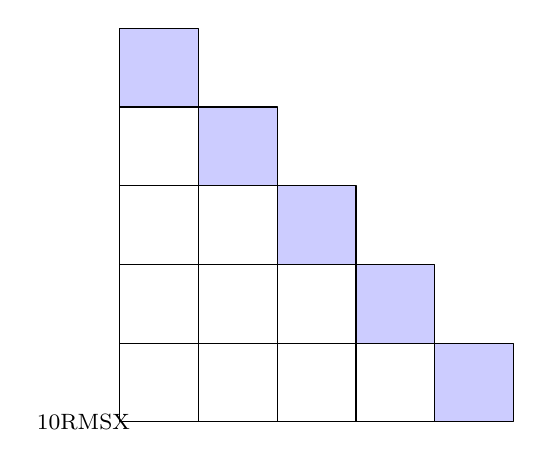
\begin{tikzpicture}[scale=1, font=\footnotesize, line join=round, line cap=round, >=stealth]
    %hidden: VM005
				\foreach \i in {1,...,5} {
				\fill[blue!20] (\i-1, 5-\i) rectangle (\i, 5-\i+1);
			}
				\foreach \r/\c in {1/5, 2/4, 3/3, 4/2, 5/1} {
				\foreach \i in {1,...,\c} {
				\draw (\i-1, \r-1) rectangle (\i, \r);
			}
			}								
    \node at (0,0){\href{10RMSX}{\tiny \phantom{10RMSX}}};
			\end{tikzpicture}
		\end{center}		
		Do nhóm $S_1$ có $5$ phần tử, ta phải xếp $5$ số này vào $5$ ô sao cho không có hai ô nào cùng hàng hoặc cùng cột. Dựa vào cấu trúc bảng bậc thang $(5, 4, 3, 2, 1)$, tập hợp duy nhất gồm $5$ ô không chung hàng và cột chính là $5$ ô nằm trên đường chéo (các ô ở vị trí ngoài cùng của mỗi cột/hàng, phần tô màu).\\		
		Ta tiến hành xếp các nhóm số vào bảng theo các bước sau:		
		\begin{enumerate}[\it B1:]
			\item Xếp $5$ phần tử của $S_1$ vào $5$ ô đường chéo. Số cách xếp $5$ số vào $5$ ô này là $5!$.
			\item Bỏ đi $5$ ô vừa xếp, phần còn lại của bảng là một bảng bậc thang $(4,3,2,1)$. Nhóm $S_2$ có $4$ phần tử, bắt buộc phải xếp vào $4$ ô không chung hàng/cột của phần còn lại này (chính là đường chéo tiếp theo). Số cách xếp là $4!$.
			\item Tương tự, bỏ đi $4$ ô vừa xếp, ta còn lại bảng $(3,2,1)$. Số cách xếp $3$ phần tử của $S_3$ vào đường chéo tiếp theo là $3!$.
			\item Phần còn lại là bảng $(2,1)$. Số cách xếp $2$ phần tử của $S_4$ vào đường chéo là $2!$.
			\item Ô cuối cùng (góc dưới cùng bên trái) duy nhất còn lại dành cho $1$ phần tử của $S_0$. Số cách xếp là $1!$.
		\end{enumerate}				
		Do đó, tổng số cách điền số thỏa mãn yêu cầu trò chơi là
		\[H = 5! \cdot 4! \cdot 3! \cdot 2! \cdot 1! = 120 \cdot 24 \cdot 6 \cdot 2 \cdot 1 = 34\,560 \text{ (cách)}. \]
		Vậy giá trị cần tính là $\dfrac{H}{10} = \dfrac{34\,560}{10} = 3\,456$.
	}
\end{ex}

\begin{ex}%[Dự án 1I9QH8-VN-MT-15+]%[2-TN-0102-BGD-2026,VM023]%[2D1H3-6]
	Một công ty nông sản có công suất chế biến không quá $180$ tấn nguyên liệu một tháng. Nếu công ty chế biến $x$ tấn nguyên liệu trong một tháng ($1 \le x \le 180$) thì chi phí sản xuất và doanh thu lần lượt là $C(x) = 0{,}002x^3 + 30x + 20$ (triệu đồng) và $R(x) = 90x$ (triệu đồng). Lợi nhuận lớn nhất mà công ty đạt được trong một tháng là bao nhiêu triệu đồng?
	\par\shortans{$3\,980$}
	\loigiai{
		Hàm số biểu diễn lợi nhuận của công ty trong một tháng là
		\[ P(x) = R(x) - C(x) = -0{,}002x^3 + 60x - 20\ \text{(triệu đồng)}. \]
		Xét hàm số $P(x)$ trên đoạn $[1; 180]$.\\
		Ta có $P'(x) = -0{,}006x^2 + 60$.\\
		Xét $P'(x) = 0 \Leftrightarrow x^2 = 10\,000 \Leftrightarrow x = 100$ (do $x \in [1; 180]$).\\
		Ta có $P(1) = 39{,}998$, $P(100) = 3\,980$, $P(180) = -884$.\\
		Vậy lợi nhuận lớn nhất công ty đạt được là $3\,980$ triệu đồng.
	}
\end{ex}

\begin{ex}%[Dự án 1ZIXYX-VN-MT-15+]%[2-TN-0102-BGD-2026,VM023]%[0C1H1-3]
	Một nông trại cung cấp rau quả cho siêu thị A với số liệu bán hàng của bốn ngày trong tuần được ghi lại trong bảng sau:
	\begin{center}
		\renewcommand{\arraystretch}{1.5}
		\begin{tabular}{|c|c|c|c|c|}
			\hline
			\multirow{2}{*}{Ngày} & \multicolumn{3}{c|}{Số ki-lô-gam} & \multirow{2}{*}{Tổng số tiền} \\ \cline{2-4}
			& Rau muống & Bí xanh & Cà chua & (nghìn đồng) \\ \hline
			Thứ Tư & $19$ & $15$ & $10$ & $615$ \\ \hline
			Thứ Năm & $20$ & $12$ & $8$ & $540$ \\ \hline
			Thứ Sáu & $25$ & $12$ & $7$ & $570$ \\ \hline
			Thứ Bảy & $50$ & $30$ & $20$ & ? \\ \hline
		\end{tabular}
	\end{center}
	Biết rằng đơn giá theo ki-lô-gam của mỗi loại rau quả trong bảng trên là không đổi. Tổng số tiền nông trại thu được ở ngày thứ Bảy từ ba loại rau quả trên khi cung cấp cho siêu thị A là bao nhiêu nghìn đồng?
	\par\shortans{$1\,350$}
	\loigiai{
		Gọi $x$, $y$, $z$ lần lượt là đơn giá một kg của rau muống, bí xanh và cà chua (nghìn đồng/kg).\\
		Dựa vào bảng số liệu, ta có hệ phương trình
		\[\heva{&19x + 15y + 10z = 615 \\&20x + 12y + 8z = 540 \\&25x + 12y + 7z = 570.}\]
		Giải hệ phương trình, ta được $x = 10$, $y = 15$, $z = 20$.\\
		Số tiền thu được của ngày thứ Bảy là
		\[ T = 50x + 30y + 20z = 50 \cdot 10 + 30 \cdot 15 + 20 \cdot 20 = 1\,350 \text{ (nghìn đồng)}. \]
	}
\end{ex}

\begin{ex}%[Dự án 65XMEV-VN-MT-15+]%[2-TN-0102-BGD-2026,VM023]%[0D0C2-6]
	\immini[thm]{Một khung hình trang trí có dạng một đa giác đều $12$ cạnh $A_1A_2\ldots A_{12}$ (xem hình vẽ) được gắn cố định trên trần nhà. Bạn Dũng có $12$ bóng đèn gồm bốn bóng màu đỏ và tám bóng màu xanh. Bạn Dũng lắp ngẫu nhiên $12$ bóng đèn vào $12$ đỉnh $A_1, A_2, \ldots, A_{12}$. Gọi $P$ là xác suất để mỗi hình vuông (có bốn đỉnh là các đỉnh của đa giác đã cho) đều có ít nhất một bóng đèn màu đỏ. Giá trị của $4\,565P$ bằng bao nhiêu?
		}{
		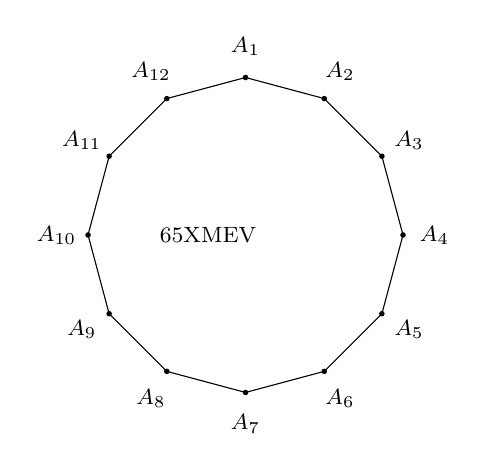
\begin{tikzpicture}[scale=1, font=\footnotesize, line join=round, line cap=round, >=stealth]
    %hidden: VM005
			\def\n{12}			
			\def\r{2}	
			\draw (90:\r) \foreach \i in {2,...,\n} { -- ({90-(\i-1)*360/\n}:\r) } -- cycle;
			\foreach \i in {1,...,\n} {
			\fill ({90-(\i-1)*360/\n}:\r) circle (1pt);				
			\node at ({90-(\i-1)*360/\n}:{\r+0.4}) {$A_{\i}$};				
			}			
    \node at (0,0){\href{65XMEV}{\tiny \phantom{65XMEV}}};
		\end{tikzpicture}
		}	
		\par\shortans{$2\,656$}
	\loigiai{
		Coi $12$ bóng đèn (gồm $4$ bóng đỏ và $8$ bóng xanh) là các phần tử đôi một phân biệt. Số cách sắp xếp ngẫu nhiên $12$ bóng đèn này vào $12$ đỉnh của đa giác đều là số hoán vị của $12$ phần tử.\\
		Do đó số phần tử của không gian mẫu là $n(\Omega) = 12!$.\\
		Đa giác đều có $12$ cạnh nên $12$ đỉnh được chia chính xác thành $3$ hình vuông độc lập, không đôi một chung đỉnh với nhau, chẳng hạn như hình dưới đây:
		\begin{center}
			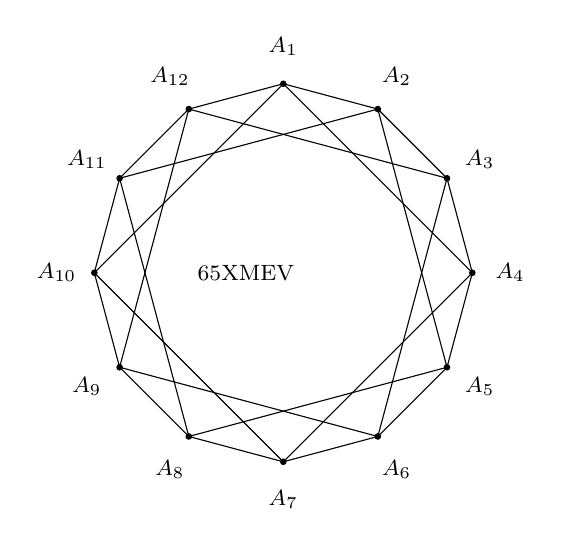
\begin{tikzpicture}[scale=1.2, font=\footnotesize, line join=round, line cap=round, >=stealth]
    %hidden: VM005
				\def\n{12}			
				\def\r{2}
				\foreach \i in {1,...,\n} {
				\coordinate (A\i) at ({90-(\i-1)*360/\n}:\r);
				\fill (A\i) circle (1pt);				
				\node at ({90-(\i-1)*360/\n}:{\r+0.4}) {$A_{\i}$};				
			}					
				\draw (A1) -- (A2) -- (A3) -- (A4) -- (A5) -- (A6) -- (A7) -- (A8) -- (A9) -- (A10) -- (A11) -- (A12) -- cycle;
				\draw (A1) -- (A4) -- (A7) -- (A10) -- cycle;
				\draw (A2) -- (A5) -- (A8) -- (A11) -- cycle;
				\draw (A3) -- (A6) -- (A9) -- (A12) -- cycle;
    \node at (0,0){\href{65XMEV}{\tiny \phantom{65XMEV}}};
			\end{tikzpicture}
		\end{center}	
		\begin{itemize}
			\item Hình vuông thứ nhất ($H_1$) gồm các đỉnh $\{A_1, A_4, A_7, A_{10}\}$.
			\item Hình vuông thứ hai ($H_2$) gồm các đỉnh $\{A_2, A_5, A_8, A_{11}\}$.
			\item Hình vuông thứ ba ($H_3$) gồm các đỉnh $\{A_3, A_6, A_9, A_{12}\}$.
		\end{itemize}
		Để mỗi hình vuông đều có ít nhất một bóng đèn màu đỏ, mà ta chỉ có tổng cộng $4$ bóng đỏ phân phối vào ba hình vuông, nên bắt buộc phải có một hình vuông chứa đúng $2$ bóng đỏ và hai hình vuông còn lại mỗi hình chứa đúng $1$ bóng đỏ.\\
		Gọi $A$ là biến cố \lq\lq Mỗi hình vuông đều có ít nhất một bóng đèn màu đỏ\rq\rq. Quy trình xếp bóng được thực hiện như sau:
		\begin{itemize}
			\item \text{Bước 1:}
			Chọn $1$ trong $3$ hình vuông để xếp $2$ bóng đỏ, có $\mathrm{C}_3^1 = 3$ cách. Chọn tiếp $2$ đỉnh trong $4$ đỉnh để đặt bóng, có $\mathrm{C}_4^2 = 6$ cách. Trong hai hình vuông còn lại, mỗi hình vuông chọn ra $1$ đỉnh trong $4$ đỉnh để đặt bóng, có $\mathrm{C}_4^1 \cdot \mathrm{C}_4^1 = 4 \cdot 4 = 16$ cách.
			\item \text{Bước 2:}
			Xếp $4$ bóng đỏ vào $4$ vị trí dành cho bóng đỏ, có $4!$ cách. Xếp $8$ bóng xanh vào $8$ vị trí trống còn lại, có $8!$ cách.
		\end{itemize}
		Số kết quả thuận lợi cho biến cố $A$ là
		\[ n(A) = (3 \cdot 6 \cdot 4\cdot 4)\cdot 4! \cdot 8! = 288 \cdot 4! \cdot 8!. \]
		Xác suất của biến cố $A$ là
		\[ \mathrm{P}(A) = \dfrac{n(A)}{n(\Omega)} = \dfrac{288 \cdot 4! \cdot 8!}{12!} = \dfrac{288 \cdot 4!}{12 \cdot 11 \cdot 10 \cdot 9} = \dfrac{32}{55}. \]
		Vậy giá trị $4\,565P = 4\,565 \cdot \dfrac{32}{55} = 2\,656$.\\
		\textit{Cách khác:} Nếu ta chỉ quan tâm đến màu sắc của các bóng đèn thì có thể giải như sau:\\
		Do $4$ bóng đèn đỏ giống nhau và $8$ bóng đèn xanh giống nhau, nên mỗi kết quả của phép thử là một cách chọn ra $4$ vị trí (đỉnh) trong $12$ vị trí của đa giác để lắp bóng đèn màu đỏ (các vị trí còn lại mặc định lắp bóng màu xanh). \\
		Số phần tử của không gian mẫu là $n(\Omega) = \mathrm{C}_{12}^4 = 495$.\\
		Gọi $A$ là biến cố \lq\lq Mỗi hình vuông (có bốn đỉnh là các đỉnh của đa giác đã cho) đều có ít nhất một bóng đèn màu đỏ\rq\rq.\\
		Các đỉnh của đa giác $12$ cạnh được chia thành $3$ nhóm, mỗi nhóm là $4$ đỉnh của một hình vuông.\\
		Để mỗi hình vuông đều có ít nhất $1$ bóng đèn màu đỏ trong tổng số $4$ bóng đỏ thì số lượng bóng đỏ được chia vào $3$ hình vuông phải theo bộ $(2, 1, 1)$.
		\begin{itemize}
			\item Số cách chọn $1$ hình vuông trong $3$ hình để nhận $2$ bóng đỏ là $\mathrm{C}_3^1 = 3$ cách.
			\item Số cách chọn $2$ đỉnh trong hình vuông đó để gắn $2$ bóng đỏ là $\mathrm{C}_4^2 = 6$ cách.
			\item Số cách chọn $1$ đỉnh trong mỗi hình vuông còn lại để gắn bóng đỏ là  $\mathrm{C}_4^1 \cdot \mathrm{C}_4^1 = 16$ cách.
		\end{itemize}
		Số kết quả thuận lợi là $n(A) = 3 \cdot 6 \cdot 16 = 288$ (đối với việc chọn vị trí, các bóng đỏ là như nhau).\\
		Xác suất cần tìm là $\mathrm{P}(A)= \dfrac{n(A)}{n(\Omega)}=\dfrac{288}{495}=\dfrac{32}{55}$.\\
		Vậy giá trị $4\,565P = 4\,565 \cdot \dfrac{32}{55} = 2\,656$.
	}
\end{ex}

\Closesolutionfile{ans}
\Closesolutionfile{ansbook}
\begin{indapan}
	{ans/ans\currfilebase}
\end{indapan}